\documentclass[11pt]{beamer}
\usetheme{Pittsburgh}
\usepackage[utf8]{inputenc}
\usepackage[english]{babel}
\usepackage{amsmath}
\usepackage{amsfonts}
\usepackage{amssymb}
\usepackage{mathrsfs} 
\usefonttheme[onlymath]{serif}
\defbeamertemplate*{title page}{customized}[1][]
{
  \usebeamercolor[fg]{titlegraphic}\inserttitlegraphic
  \flushleft
  \medskip
  \usebeamerfont{title}\inserttitle\par
  \medskip
  \usebeamerfont{subtitle}\usebeamercolor[fg]{subtitle}\insertsubtitle\par
  \vfill
  \usebeamerfont{author}\insertauthor\par
  \usebeamerfont{institute}\insertinstitute\par
  \medskip
  \usebeamerfont{date}\insertdate\par

}

\titlegraphic{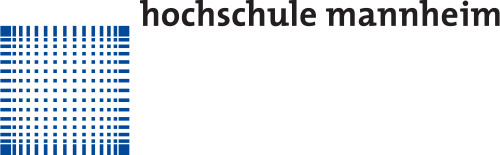
\includegraphics[scale=0.25]{logo.png}}
\author{Horst Schneider, Patrick Beedgen}
\title{Understanding Eventual Consistency}
\subtitle{MSI Presentation SS2014}
\institute{Hochschule Mannheim} 
\date{June 17th, 2014} 
\begin{document}

\begin{frame}
\titlepage
\end{frame}

%\begin{frame}
%\tableofcontents
%\end{frame}

\begin{frame}
\frametitle{Introduction}
\begin{quotation}
\glqq ...the 
storage system guarantees that if no 
new updates are made to the object, 
eventually all accesses will return the 
last updated valuee\grqq
\linebreak
--W. Vogels (2009)
\end{quotation}

\begin{quotation}
\glqq Zweites Zitat über Ev. Consistency \grqq
\end{quotation}
\end{frame}

\begin{frame}
\frametitle{The Problem}
\begin{itemize}
  \item The definitions are ambiguous\linebreak
  \item Most big players claim to implement it\linebreak
  \item Implementations can't be be compared\ldots scientifically

\end{itemize}
\end{frame}

\begin{frame}
\frametitle{Anfang Hauptteil Horst}
\end{frame}

\begin{frame}
\frametitle{Replicated Data Types}
\begin{itemize}
\item A replicated database stores \textbf{objects} \(\mathrm{Obj} = \{x,y,\dots\} \)
\pause
\item Every object \(x \in \mathrm{Obj}\) has
\begin{itemize}
\item a \textbf{value} \(\in \mathrm{Val}\)
\pause
\item a \textbf{type} type\((x)\)
\pause
\item  \textbf{operations} \(\mathrm{Op}_{\mathrm{type}(x)}\) that a client can perform on it
\pause
\end{itemize}
\item Two examples: Int Register \textbf{intreg}, Counter \textbf{ctr}
\end{itemize}

\begin{align*}
\mathrm{Op}_\mathrm{ctr} &= \mathrm{\{rd, inc\}} \\
\mathrm{Op}_\mathrm{intreg} &= \mathrm{\{rd, wr(}k \mathrm{)|} k \in \mathbb{Z} \mathrm{\}}
\end{align*}
\end{frame}

\begin{frame}
\frametitle{Replicated Data Types}
\framesubtitle{Sequential Data Type Specification}
In a \textit{strongly consistent system}, the semantics of a data type can be described by a function \\
\begin{equation*}
S_{\tau}\ : \mathrm{Op}_\tau^+ \rightarrow \mathrm{Val}
\end{equation*}
\pause
Examples:
\begin{align*}
S_{\mathrm{ctr}} \mathrm{(\sigma rd)} &= \mathrm{(number\ of\ inc\ operations\ in\ \sigma);} \\
\onslide<3->{S_{\mathrm{intreg}} \mathrm{(\sigma rd)} &= k;\ \mathrm{if\ wr(0) \sigma = \sigma_1 wr(}k\mathrm{) \sigma_2\ and} \\
 & \mathrm{\sigma_2 \ does\ not\ contain\ wr\ operations} \\}
\onslide<4->{
S_{\mathrm{intreg}} \mathrm{(\sigma\ wr(}k\mathrm{))} &= S_{\mathrm{ctr}} \mathrm{(\sigma\ inc)} = \bot; }
\end{align*}
\end{frame}

\begin{frame}
\frametitle{Replicated Data Types}
\framesubtitle{Conflict Resolution Strategies}

\begin{columns}
\begin{column}{5cm}
\begin{figure}
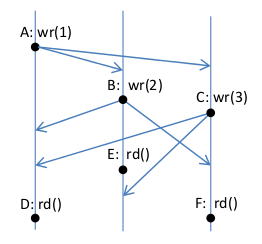
\includegraphics[scale=0.6]{update_replicas.png}
\end{figure}
\end{column}
\begin{column}{5cm}
\pause
\begin{enumerate}
\item Make concurrent operations commutative
\pause
\item Order concurrent operations
\pause
\item Flag conflicts (let the user decide)
\pause
\item Resolve conflicts semantically
\end{enumerate}
\end{column}
\end{columns}
\end{frame}

\begin{frame}
\frametitle{Replicated Data Types}
\framesubtitle{Replicated Data Type Specification}
\begin{itemize}
\item \(S_{\tau}\) is not strong enough to formalize these strategies
\pause
\item visibility and order of preceding operations have to be included
\pause
\item \(F_\tau\): takes an \textbf{operation context} and returns a \textbf{value}
\end{itemize}

\begin{center}
\(F_\tau(C) \in \mathrm{Val}\) \\
\end{center}
\pause
\begin{itemize}
\item operation context \(C\) adds \textbf{visibility} and \textbf{arbitration relations} to preceding operations:
\end{itemize}

\begin{center}
\(C = (f, V, \mathrm{ar}, \mathrm{vis})\) \\
\pause
\(u \xrightarrow{\mathrm{vis}} v, \mathrm{vis} \subseteq V \times V  \) \\
\pause
\(u \xrightarrow{\mathrm{ar}} v, \mathrm{ar} \subseteq V \times V  \)
\end{center}

\end{frame}

\begin{frame}

\end{frame}

\begin{frame}
\frametitle{Ende Hauptteil Horst}
\end{frame}

\begin{frame}
\frametitle{Anfang Hauptteil Patrick}
\end{frame}


\begin{frame}
\frametitle{Ende Hauptteil Patrick}
\end{frame}


\begin{frame}
\frametitle{Conclusion}
\begin{itemize}
\item Which problems does the techreport solve?
\item What is not solved by it?
\item What do \textbf{we} think about it?
\end{itemize}
\end{frame}

\end{document}
